\documentclass[onecolumn, draftclsnofoot,10pt, compsoc]{IEEEtran}
\usepackage{graphicx}
\usepackage{url}
\usepackage{setspace}

\usepackage{geometry}
\geometry{textheight=9.5in, textwidth=7in}


% 1. Fill in these details
% 1. Fill in these details
\def \CapstoneTeamName{		Team TriTone}
\def \CapstoneTeamNumber{		045}
\def \GroupMemberOne{			Christopher Hebert}
\def \GroupMemberTwo{			Aidan O'Malley}
\def \GroupMemberThree{			Kazuriah Buckley}
\def \CapstoneProjectName{		Interactive Music Theory Application}
\def \CapstoneSponsorPerson{		Lukas Hein}

% 2. Uncomment the appropriate line below so that the document type works
\def \DocType{		%Problem Statement
				%Requirements Document
  Technology Review
				%Design Document
				%Progress Report
				}
			
\newcommand{\NameSigPair}[1]{\par
\makebox[2.75in][r]{#1} \hfil 	\makebox[3.25in]{\makebox[2.25in]{\hrulefill} \hfill		\makebox[.75in]{\hrulefill}}
\par\vspace{-12pt} \textit{\tiny\noindent
\makebox[2.75in]{} \hfil		\makebox[3.25in]{\makebox[2.25in][r]{Signature} \hfill	\makebox[.75in][r]{Date}}}}
% 3. If the document is not to be signed, uncomment the RENEWcommand below
%\renewcommand{\NameSigPair}[1]{#1}

%%%%%%%%%%%%%%%%%%%%%%%%%%%%%%%%%%%%%%%
\begin{document}
\begin{titlepage}
    \pagenumbering{gobble}
    \begin{singlespace}
    	
\includegraphics[height=4cm]{coe_v_spot1}
        \hfill 
        % 4. If you have a logo, use this includegraphics command to put it on the coversheet.
        %\includegraphics[height=4cm]{CompanyLogo}   
        \par\vspace{.2in}
        \centering
        \scshape{
            \huge CS Capstone \DocType \par
            {\large\today}\par
            \vspace{.5in}
            \textbf{\Huge\CapstoneProjectName}\par
            \vfill
            {\large Prepared by }\par
            \vspace{5pt}
            {\Large
                \NameSigPair{\GroupMemberOne}\par
            }
            \vspace{20pt}
        }
        \begin{abstract}
          This document outlines several technology-related design decisions specifically about the composition page.
          Methods for chord entry, chord editing, and composition analysis are discussed. 
          Decisions are made about which technologies to choose.
        \end{abstract}     
    \end{singlespace}
\end{titlepage}
\newpage
\pagenumbering{arabic}
\tableofcontents
% 7. uncomment this (if applicable). Consider adding a page break.
\listoffigures
%\listoftables
\clearpage

% 8. now you write!

\section{Introduction}
This document evaluates different design and technological decisions for chord entry, composition editing, and analysis.
This app will exist in a saturated market, so there are plenty of examples of how other applications handle this set of design choices.
Sibelius 7 is a popular application to design musical scores.
It allows for chord entry using plain-English text entry, direct MIDI note entry, and it can also calculate chord name and quality from a group of notes.
\cite{sibelius}
GarageBand is an app for creating music on iOS devices.
It allows for chord entry using a Chord Wheel.
\begin{figure}[h]
  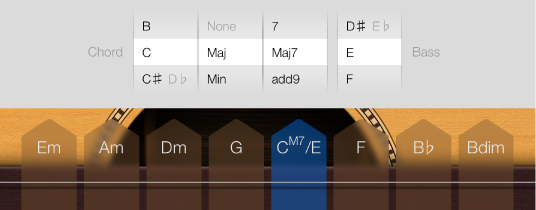
\includegraphics[width=0.25\textwidth]{garageband.png}
  \caption{Image of GarageBand's Chord Wheel from \cite{garageband}.}
\end{figure}
\cite{garageband}
Chord! is an iPhone and iPad app that is designed to help with music composition.
Chord! is interesting because it uses analysis to help the user enter chords.
Chord! claims that it ``uses [music theory] to give more meaningful and accurate results in a way that you can understand too the underlying theory.''
\begin{figure}[h]
  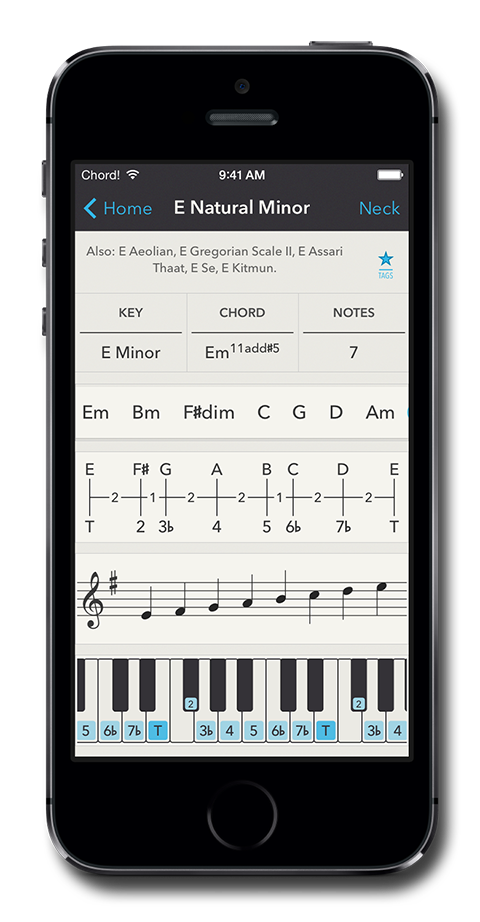
\includegraphics[width=0.25\textwidth]{chord.png}
  \caption{Image of Chord!'s music theory analysis from \cite{chord}.}
\end{figure}
\cite{chord}
All of these apps are designed for writing and composing music,
and have tools specific to the composition style for editing chords individually.
Sibelius 7 and GarageBand allow users to edit chords by editing the notes.
Chord! allows users to edit chords individually using a combination of analysis, radio buttons, and check boxes.

\section{Composition Page: Chord Entry}
\subsection{Overview}
In order for users to create compositions they need to be able to enter chords. 
These chords will be based on a root tone and need to have a specific quality. 
The mechanism for chord entry should be able to handle: 
choosing a root tone from one of the 12 tones, 
choosing minor or major chord quality, 
and choosing whether the 7th is present and its quality. 
Intervals other than the 7th are outside the scope of this application. 
\subsection{Criteria}
The criteria for choosing which chord entry style to use will include:
accuracy of user input,
ease of recovering from mistakes in user input,
cohesion with the other parts of the app,
complexity of implementation.

\subsection{Potential Choices}
\subsubsection{Keyboard Style Chord Entry}
\begin{figure}[h]
  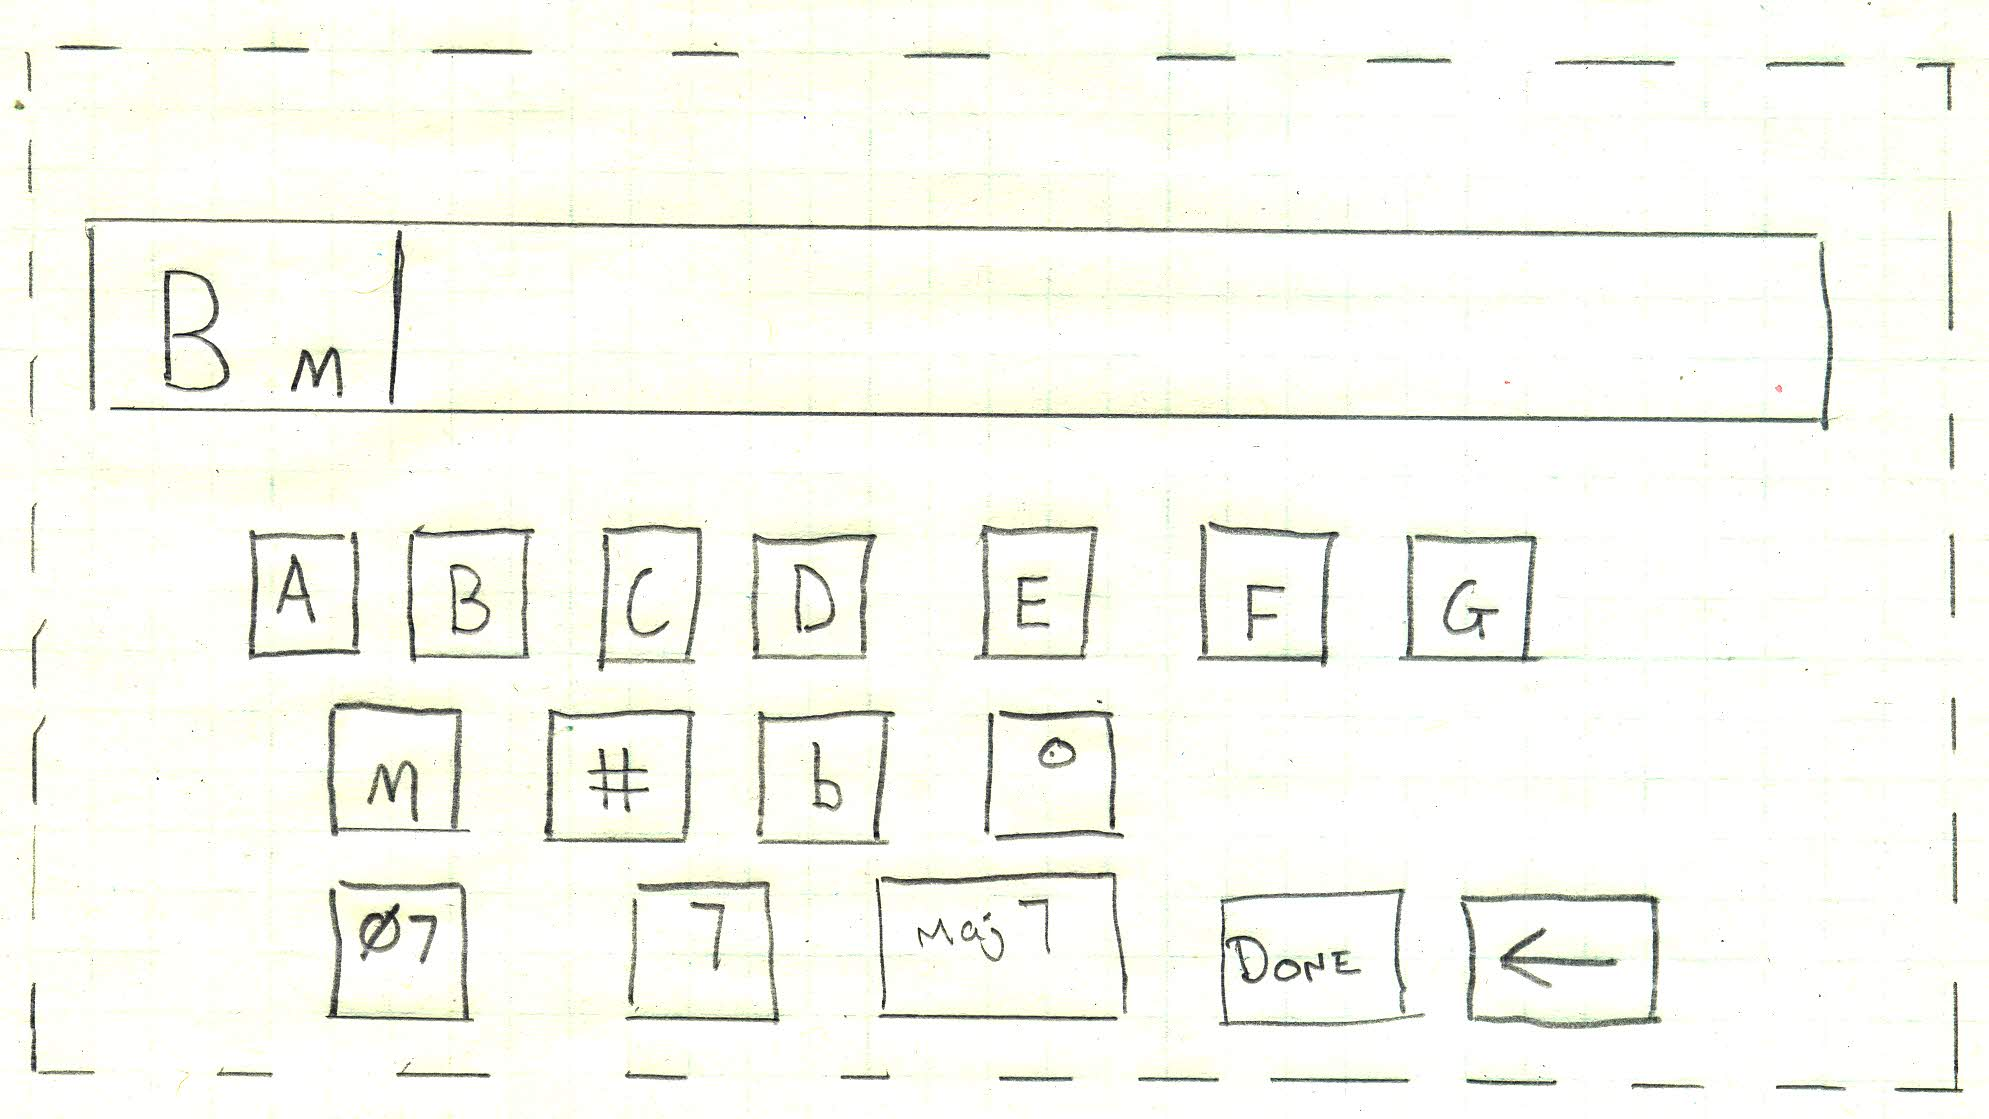
\includegraphics[width=0.5\textwidth]{keyboard.png}
  \caption{User in the process of entering ``Bm7'' using keyboard-style chord entry.}
\end{figure}

The keyboard style chord entry would have a text area for writing out the chords, as well as a grid layout of buttons for chord entry. 
The grid of buttons would contain note names, qualities, and intervals. 
For example, if the user wanted to enter "B minor 7th", they would push "B", "m", "7" buttons in that order, and the text area would be populated with "Bm7". 

\subsubsection{Circle of Fifths Style Chord Entry}
\begin{figure}[h]
  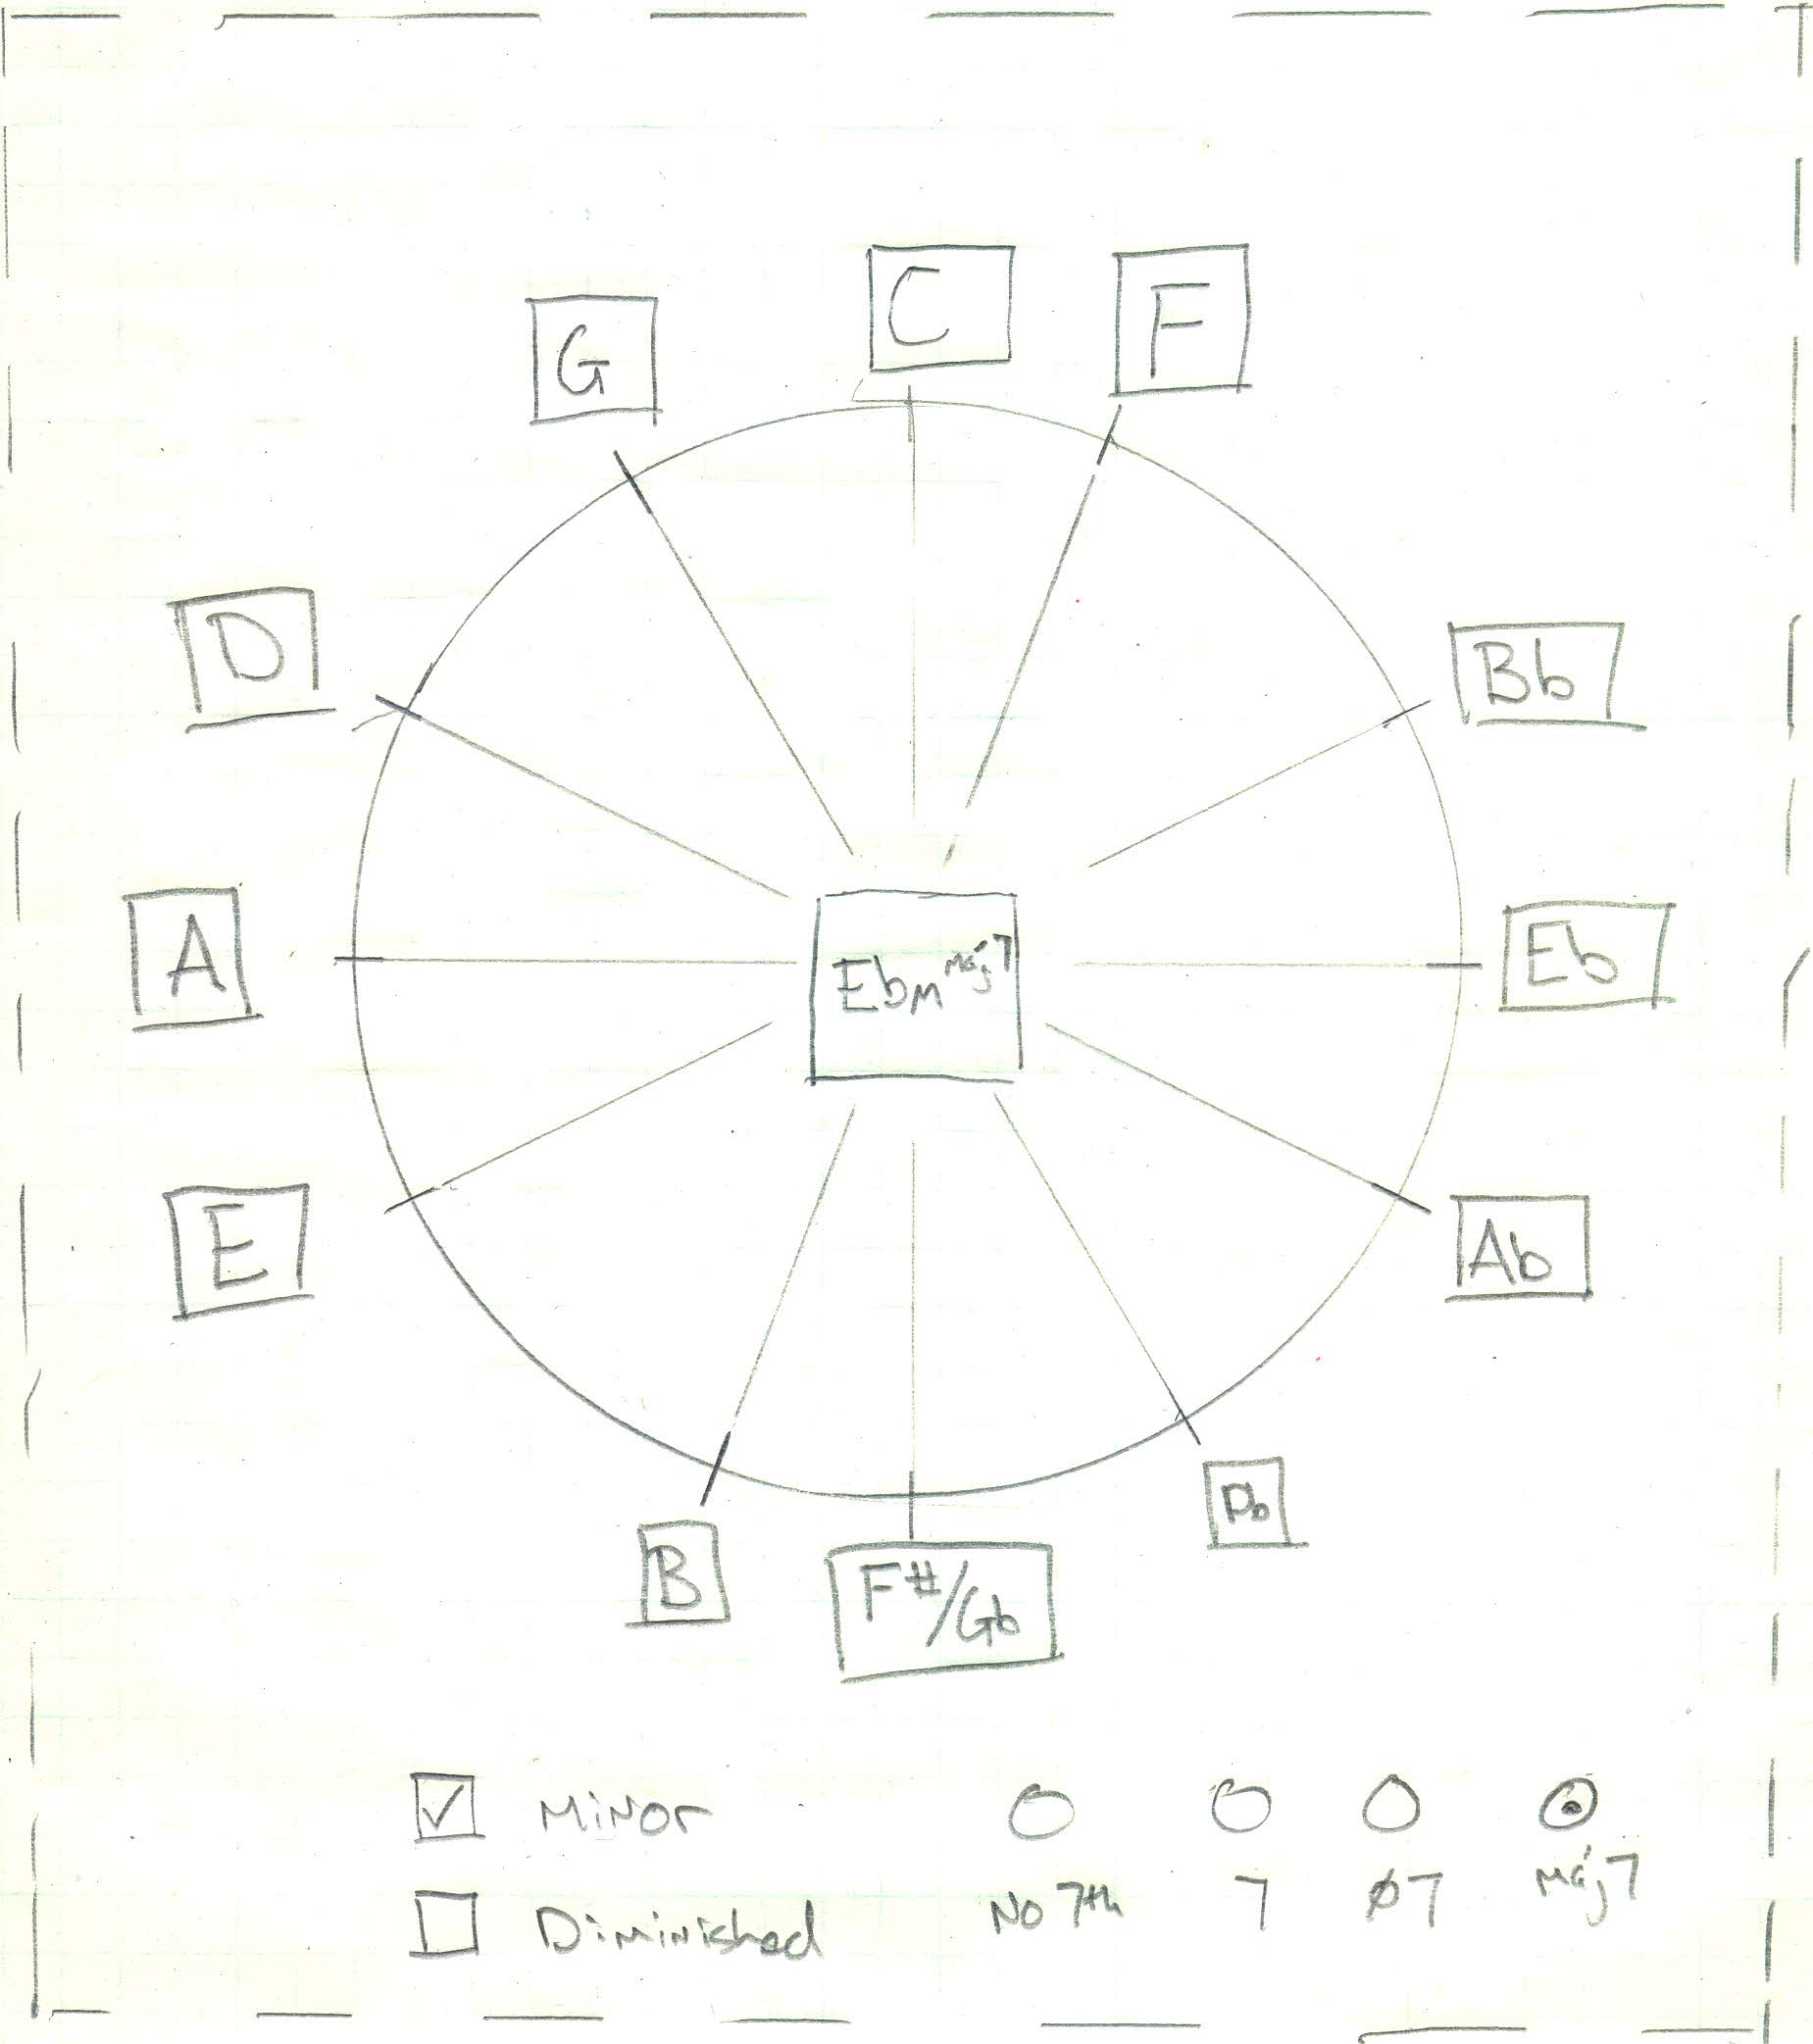
\includegraphics[width=0.5\textwidth]{circle.png}
  \caption{User has chosen the chord ``Ebm Maj7'' using the Circle of Fifths-style chord entry.}
\end{figure}

The circle of fifths style chord entry would use a circle of fifths for tone entry, as well as two groups of radio buttons for chord quality and 7th interval quality.
The user would touch any of the notes on the circle of fifths to determine the root tone of the chord. 
The chord quality radio buttons would be either major or minor. 
The 7th interval quality could be none, 7th, major 7th, or diminished 7th. 

\subsubsection{Grid of Radio Buttons}
\begin{figure}[h]
  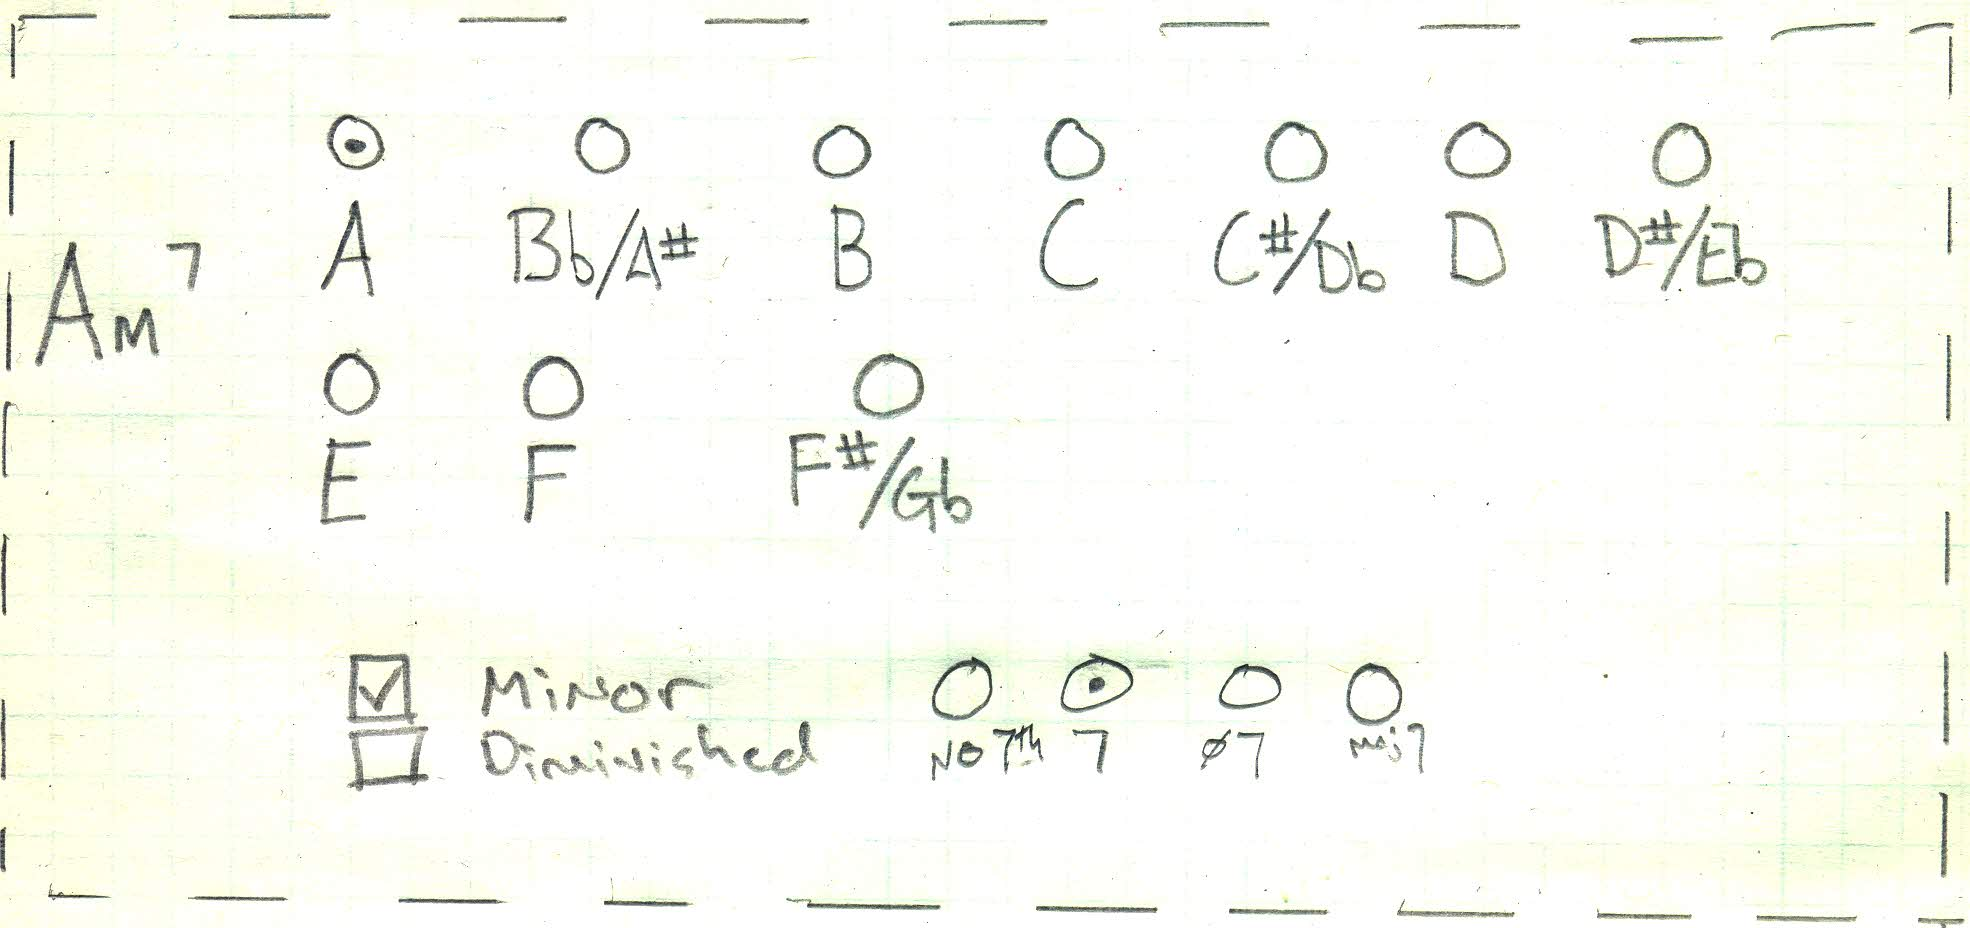
\includegraphics[width=0.5\textwidth]{radio.png}
  \caption{User has entered the chord ``Am7'' using the grid of radio buttons-style chord entry.}
\end{figure}

The third choice uses: a set of radio buttons to determine tone, a set of radio buttons to determine chord quality, and a set of radio buttons to determine the presence and quality of the 7th. 
\subsection{Discussion}
All three methods allow the user to input chords accurately and with a preview.
Keyboard-style entry could allow for invalid chords to be entered, and therefore requires the most work when recovering from user input error.
The other two methods don't allow for invalid chord names to be entered.
The Circle of Fifth's method of chord entry has very high cohesion with the other part of the app: the Circle of Fifth's page.
This would allow users to develop muscle and spatial memory of the Circle of Fifth's as they practice composing.
The keyboard style entry would be the most complex to implement.
Keyboard style entry would need:
a text entry box,
a cursor that can navigate in the text entry box,
key entry,
deletion,
and tests to make sure that the chord entered was valid.
The other two entry methods only allow valid chord entries, and are made up of radio buttons and check boxes.

We will be implementing the Circle of Fifths style chord entry, 
since it solves the problem simply and effectively,
and has the added benefit of drilling muscle memory for users,
and has high cohesion with other parts of the app.

\section{Composition Page: Composition Editing}
\subsection{Overview}
As users create compositions they may realize that they want to make a change to a chord that is already in the composition.
Editing chords means that the user starts with a composition that they don't want, and ends up with a composition that they do want (or at least thought that they wanted).
Compositions will be short enough to be visible on a single page.
Tools to analyze, and edit will also be on this same page.

\subsection{Criteria}
The criteria for choosing chord editing will be:
ease of use,
ease of learning,
ease of implementation,
and how much visual clutter to the interface the editing style adds.

\subsection{Potential Choices}
\subsubsection{Chords are Implemented as Text Elements with Touch Events}
Having chords in a composition as text elements gives them the appearance of being plain text. 
They can be drawn in sequence. 
In order to make them editable, they will have a touch event registered to them. 
When the user touches them, the event will trigger the chord entry to begin changing the chord that the user touched. 
\subsubsection{Chords are Implemented as Buttons}
In this scenario the chords are implemented as buttons. 
It will be obvious to the user that something will happen if they push the chord buttons. 
When the user pushes a button, chord entry will begin and the user can change the chord that she or he picked. 
\subsubsection{Chords are Implemented as Text Elements}
In this scenario, the chords are implemented as text elements, but they are not directly editable. 
If the user wishes to change the composition, he or she can remember the composition they were editing and start a new one with the change implemented. 
There will be a button which will discard the old composition and create a new one, and will be labeled to indicate this.
\subsection{Discussion}
The first two are the easiest for editing compositions.
These give the user the tools to change only one chord at a time.
The second and third options are easiest to learn.
It is not obvious that text elements are buttons, but it is obvious that something will happen with the user presses one of the buttons.
\cite{uxplanet}
The third option is easier to learn, since the button to change the composition will be labeled.
The third option is the easiest to implement.
It only has one button which discards the current composition.
The other two implementations have about the same complexity of implementation one button or touch event for each chord.
The first two options add several new touchable elements.
Since touchable elements should be larger, this would increase the visual clutter.
\cite{apple}

In conclusion we will be implementing the chords as text elements, without direct edit-ability. 
This choice is the simplest, and matches the goals of the app the best. 
The purpose of the composition page is to demonstrate the rules of the schedule of tonal gravity. 
Once users have a solid foundation in these rules, they won't have much need for the composition portion of the app. 
 
\section{Composition Page: Analysis}
\subsection{Overview}
The purpose of the composition page is to analyze user compositions according to the rules of the Schedule of Tonal Gravity (henceforth referred to as "the rules").
The rules either apply to the first chord, or a transition between two chords.
Therefore, analysis requires at most a chord and its subsequent chord to determine a meaningful result.
The purpose of this section is to determine trade-offs in when and how much of the compositional analysis is performed.

\subsection{Criteria}
The criteria for determining the style for analysis include:
flexibility of use,
ease of understanding,
amount of visual clutter.

\subsection{Potential Choices}
\subsubsection{User Picks a Single Chord to Have Analyzed}
\begin{figure}[h]
  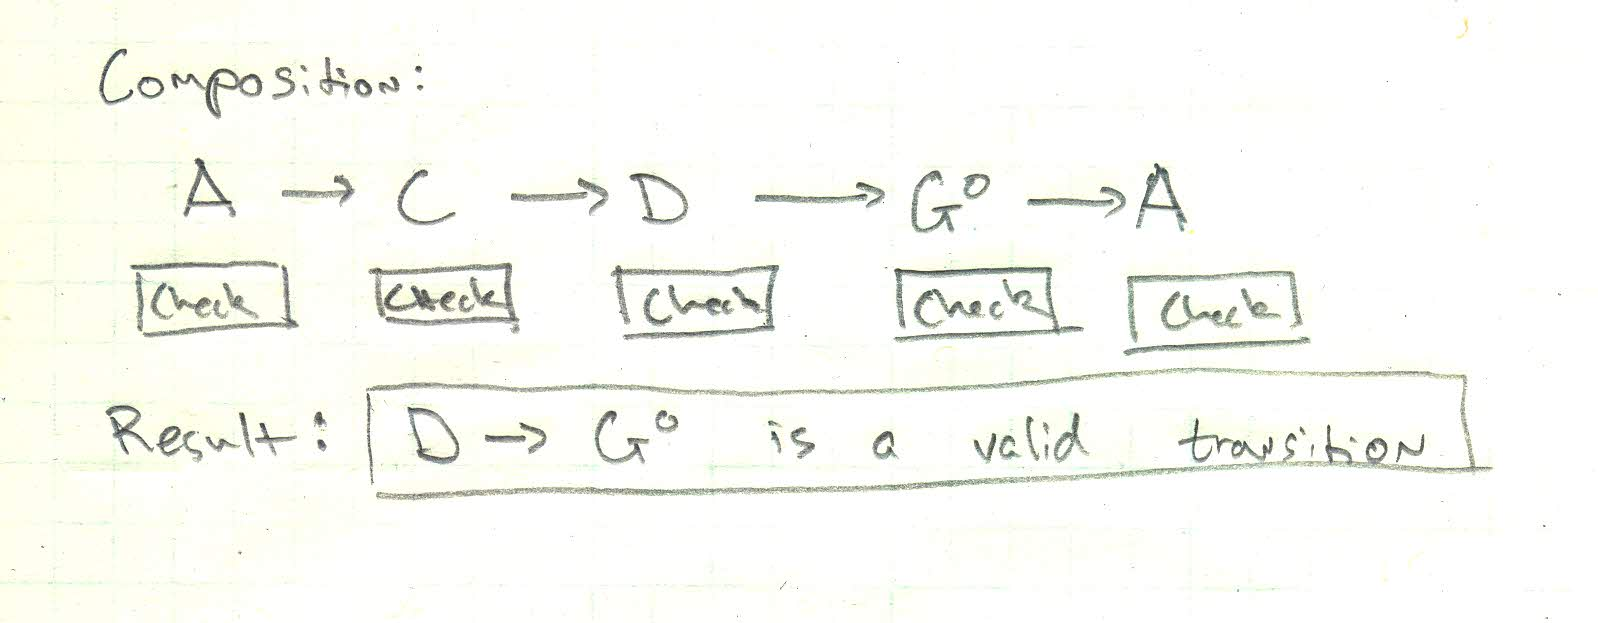
\includegraphics[width=0.5\textwidth]{analyze-each.png}
  \caption{The user has pressed the ``Check'' button associated with G diminished in the single chord analysis-style.}
\end{figure}

In this scenario the user would push a button closely associated with the chord they would like to have analyzed. 
The chord would be compared to the previous chord (or no chord, in the case of the first chord) to determine whether the chord was a valid choice.
There would be a result text-area to show the result of the single analysis.
\subsubsection{Entire Composition is Analyzed}
\begin{figure}[h]
  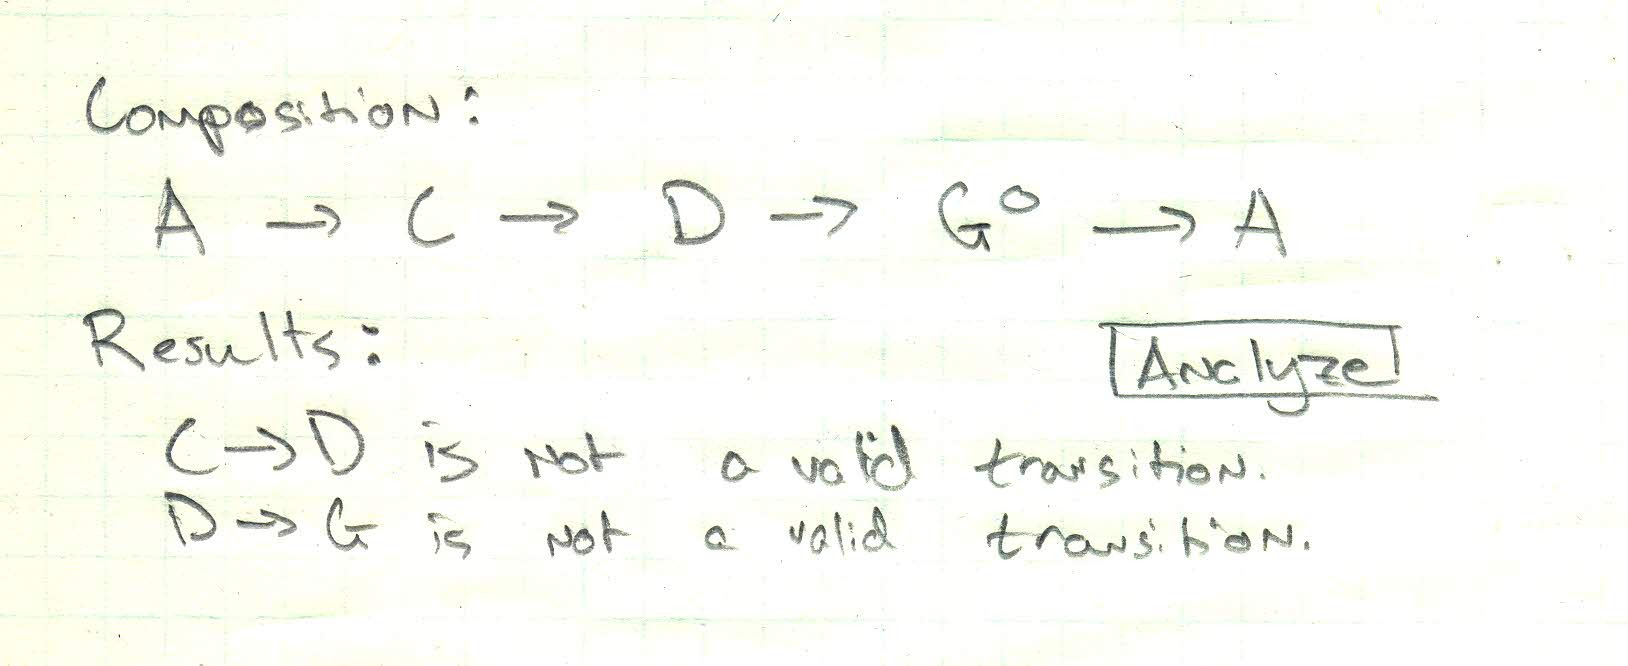
\includegraphics[width=0.5\textwidth]{analyze-all.png}
  \caption{The results section is populated with all of the broken rules in the composition in the entire composition analysis-style.}
\end{figure}

In this scenario, the user would push a button that would analyze or re-analyze the entire composition,
looping over each chord and pair of chords to determine which followed the rules.
There would be a results text-area which would contain a list of all of the transitions that violated the rules.
\subsubsection{Composition is Analyzed when Chord is Added or Changed}
If a chord is added, that chord would immediately be analyzed.
If a chord is changed, that chord, as well as the subsequent chord, would be re-analyzed. 
The results text-area would be updated to reflect the new analysis.
\subsection{Discussion}
The first option is the most flexible. 
It allows the user to not immediately receive feedback, if they wanted to do their own analysis.
It allows the user to specify exactly which chord or chord transition they want analyzed.
The second option has less flexibility.
The user is able to not receive feedback, but they only have the ability to analyze the whole song at once.
The third option provides the user with the least flexibility, forcing them to receive feedback whenever a chord is entered.

The third option is the easiest to understand, since it does not require any special input from the user.
All analysis is performed automatically.
The second option is the also easier to understand, since there is only one button to analyze the entire song,
and the user doesn't need to know about how analysis works.
The first option could be considered simpler, since the user would immediately know which chord transition posed a problem.

The first option creates the most clutter, since an additional button would need to exist for each chord in the composition.
The second option would create a bit more clutter than the third option, but only a single button.

We will be implementing the entire composition being analyzed at the push of a button (choice 2).
This maintains enough user flexibility without cluttering the UI. It is also still very easy to understand.

\section{Conclusion}
The market for apps of this nature may be saturated, but that doesn't mean that we don't need to do our own design work.
The trade-offs we have made for our design decisions are very much specific to the app we are designing.
We chose the Circle of Fifths method of chord entry to mesh with the main page and thrust of our app.
We chose to have compositions be short and simple, to encourage users to start writing down their compositions in their own way.
We chose to have editing of compositions be wholesale to give students new opportunities for creativity.
We chose to have delayed analysis of composition to give users, who will be using the app to learn music theory, an opportunity to think through the problem themselves.
All of these design choices could have been completely different if any of the goals of the app were changed.

\begin{thebibliography}{9}
\bibitem{apple}
  \textit{UI Design Do's and Don'ts,}
  \\\texttt{https://developer.apple.com/design/tips/}

\bibitem{chord}
  Thomas Grapperon.
  \textit{Chord! The Definitive Guitar App}
  \\\texttt{http://getchord.com/}
  2014
  
\bibitem{garageband}
  \textit{Garage Band for iPad: Add Your Own Custom Chords}
  \\\texttt{https://help.apple.com/garageband/ipad/2.3/\#/chsab9d1c4c}

\bibitem{sibelius}
  \textit{Sibelius 7 Tutorials}
  \\\texttt{http://hub.sibelius.com/download/documentation/pdfs/sibelius713-tutorials-en.pdf}

\bibitem{uxplanet}
  Nick Babich.
  \textit{Button UX Design: Best Practices, Types, and States,}
  \\\texttt{https://uxplanet.org/button-ux-design-best-practices-types-and-states-647cf4ae0fc6?gi=bc6cdbd6bca1}
  March 15, 2016
  
\end{thebibliography}

\end{document}
